\clearpage
\textbf{ГЛАВА 3. Практический анализ и сравнение источников энтропии}

\textbf{3.1. Сравнительный анализ источников энтропии}

Сравнение различных физических и квантовых источников энтропии
показывает, что каждый из них обладает уникальными преимуществами и
ограничениями, что делает их пригодными для разных сфер применения в
зависимости от конкретных требований к качеству случайности, уровню
безопасности, потребляемым ресурсам и технологическим возможностям
интеграции.

Физические источники энтропии, такие как тепловой шум, дробовой шум,
лавинный шум и мерцающий шум, характеризуются относительно простой
схемотехнической реализацией и возможностью интеграции в существующие
полупроводниковые платформы. Это делает их особенно привлекательными для
встраивания в микроконтроллеры, криптографические процессоры и другие
устройства массового производства. Однако такие источники могут быть
чувствительны к температурным колебаниям, электромагнитным наводкам,
старению компонентов и другим нежелательным факторам, которые могут
вносить детерминированные искажении в сигнал, снижая истинную энтропию.
Например, тепловой шум достаточно стабилен, но имеет сравнительно низкую
энтропийную мощность, что ограничивает его скорость генерации. Дробовой
и лавинный шумы более насыщены энтропией и менее предсказуемы, но
требуют сложной схемы усиления и фильтрации, а также могут генерировать
импульсные сигналы, неравномерные по амплитуде и длительности. Мерцающий
шум отличается высокой интенсивностью при низких частотах, но сложен для
оценки и контроля, а также может быть подвержен воздействию окружающей
среды.

Квантовые источники энтропии, основанные на таких явлениях, как
квантовые переходы, туннелирование, спонтанное излучение или рассеяние
фотонов, обеспечивают наивысший уровень истинной случайности, поскольку
происхождение сигнала невозможно описать детерминированными законами
физики. Это делает такие источники предпочтительными для задач, где
требуется абсолютная непредсказуемость, например, в генерации ключей для
квантово-устойчивой криптографии. Однако их реализация требует
прецизионной оптики, фотонных детекторов, лазеров или других сложных
квантово-оптических компонентов. Это не только увеличивает стоимость
устройств, но и требует особых условий эксплуатации, включая защиту от
вибраций, температурную стабилизацию и экранирование от внешних
воздействий. Кроме того, из-за высокой чувствительности к шумам и дрейфу
параметров оборудования, такие системы нуждаются в регулярной калибровке
и контроле качества работы.

Макроскопические и хаотические источники энтропии основаны на трудно
моделируемых динамических процессах, таких как движение в турбулентных
потоках, случайные колебания в нелинейных цепях или шум в радиоэфире.
Они интересны прежде всего своей простотой в реализации и возможностью
достигать очень высокой скорости генерации, что особенно полезно для
приложений, не связанных с криптографией, но требующих большого
количества случайных данных (например, в компьютерных играх или
симуляционных моделях). Однако эти источники страдают от высокой
зависимости от внешних условий и трудно поддаются строгой математической
верификации, что делает их менее надёжными в задачах, где требуется
доказуемо высокая энтропия. Кроме того, при известной модели системы, в
теории, возможно частичное предсказание поведения хаотического
источника, особенно если используется псевдослучайный усилитель
динамики.

В обобщении, можно сказать, что физические источники -- это компромисс
между простотой, скоростью и надёжностью, квантовые -- максимум
безопасности и непредсказуемости при высокой стоимости, а хаотические --
высокая производительность при умеренном уровне доверия. Поэтому выбор
зависит от того, что критично в конкретной системе: высокая скорость,
минимальные затраты, интегрируемость или гарантированная случайность.

\textbf{3.2. Архитектура экспериментального стенда и программная инфраструктура}

Практическая часть работы опирается на выделенную подсистему сбора и анализа
данных генераторов истинно случайных последовательностей на базе микроконтроллера
семейства Arduino и набора программ для персонального компьютера. Инфраструктура
спроектирована модульно: для каждого физического канала энтропии задаются отдельная
прошивка и описание аппаратной обвязки, но формат представления выборок на стороне
ПК, цепочка постобработки и статистические процедуры едины. Такой подход допускает
сравнение источников при одинаковых условиях регистрации и верификации и упрощает
включение новых каналов без переписывания общего контура измерений.

\textbf{3.2.1. Назначение и модульная организация}

Стенд предназначен для натурной регистрации потоков отсчётов аналого-цифрового
преобразователя, их сохранения в виде воспроизводимых двоичных массивов, первичной
постобработки с получением битовых последовательностей и последующего статистического
контроля --- вплоть до запуска эталонного пакета NIST Statistical Test Suite. Логически
выделяют уровень измерительного узла на микроконтроллере с первичным датчиком, уровень
протокола последовательного канала, уровень программ захвата и метаданных на
хост-компьютере, уровень численного анализа и отчётности, а также уровень
формализованной проверки случайности по методикам NIST. Схемные решения, перечень
элементов и правила безопасной сборки приведены в технической документации по каждому
каналу и сопоставлены с теоретическими разделами главы~2 без воспроизведения здесь
полного комплекта чертежей и расчётов.

\textbf{3.2.2. Аппаратная часть и прошивки микроконтроллера}

Используется компактная плата на микроконтроллере ATmega328P со встроенным
десятиразрядным АЦП и высокоскоростным преобразователем USB--UART. Аналоговые источники
энтропии подключаются к линиям входа АЦП; цифровые датчики доступны по шине
I$^2$C с последующей упаковкой считываемых регистров в единый числовой формат отсчётов,
совместимый с остальными каналами. Реализованный набор охватывает тепловой шум на
резисторе, лавинно-дробовые режимы полупроводниковых приборов, акустический модуль на
электретном капсюле, MEMS-инерциальный датчик, режим «плавающего» входа АЦП для учёта
наводок, оценку дрожания тактов относительно сторожевого таймера, а также гибридную
комбинацию нескольких каналов с последующим смешением на стороне ПК.

Для каждого варианта предусмотрен отдельный скетч прошивки. Общие конструкции ---
формализованное описание последовательного протокола и процедуры ускоренного режима
выборки АЦП --- вынесены в разделяемые заголовочные файлы и подключаются всеми
конфигурациями. При записи программы в память контроллера задаются символьный
идентификатор источника, номинальная частота дискретизации, число используемых бит
динамического диапазона при выбранном опорном напряжении и поясняющая строка об
аппаратной конфигурации; эти поля затем автоматически попадают в метаданные сеанса на
компьютере и используются при интерпретации спектральных графиков и скорости потока.

\textbf{3.2.3. Протокол обмена и программы захвата}

После сброса микроконтроллер передаёт короткий текстовый блок служебных строк с
ключами параметров формата (\textit{little-endian}, беззнаковые 16-битные слова),
частотой опроса АЦП, типом опоры преобразователя и произвольным комментарием к навесным
элементам; за маркером начала двоичной фазы следует непрерывный поток двухбайтовых слов
без разбиения на пакеты фиксированной длины. Скорость линии последовательного интерфейса
выбирается повышенной (порядка одного мегабита в секунду), что задаёт верхнюю границу
пропускной способности канала совместно с ограничениями быстродействия АЦП и цикла
прерываний прошивки.

На стороне ПК выполняется приём потока из COM-порта: текстовая преамбула отделяется от
двоичной части, последняя сохраняется как массив отсчётов фиксированного формата, а
параметры из преамбулы сериализуются рядом с дампом для автоматического использования при
построении спектров и вычислении длительности записи по объёму данных и временным
меткам приёмника.

\textbf{3.2.4. Обработка на персональном компьютере и формирование отчётов}

Далее из массива отсчётов извлекаются выбранные младшие двоичные разряды с образованием
упакованного битового файла; опционально выполняется постобработка по схеме фон Неймана.
Отдельные программные модули строят гистограмму уровней, оценивают спектральную плотность
методом Уэлча, вычисляют автокорреляцию выборок или битов, оценивают энтропию на символ в
терминологии, согласованной с NIST SP~800-90B, и формируют растровое изображение фрагмента
битового потока заданного размера. Итоговый сценарий собирает графические файлы и
числовые сводки в единый текстовый отчёт по каждому источнику, из которого удобно
переносить таблицы и иллюстрации в рукопись работы.

Имеется объединяющий конвейерный сценарий, последовательно запускающий захват при
подключённом узле, постобработку, построение отчёта и при необходимости статистические
тесты --- это уменьшает риск расхождения версий данных между этапами и облегчает повтор
эксперимента на том же аппаратном комплекте.

\textbf{3.2.5. Интеграция с пакетом NIST STS}

Для формализованной проверки двоичных последовательностей подключается реализация
NIST STS версии 2.1.2: подготовленные двоичные файлы подаются на вход утилиты оценки,
выходные таблицы преобразуются в компактное представление с долями успешных потоков по
каждому типу теста и агрегированными вердиктами. Эта ступень дополняет теоретический
материал главы~1 практической иллюстрацией: расхождение результатов для «сырых» бит и для
последующности после фон Неймана, а также появление статусов «не применимо» у отдельных
групп тестов при выраженном смещении входного потока отражают свойства данных и области
применимости конкретных критериев пакета, а не ошибку связки аппаратуры с программами.

\textbf{3.3. Натурная оценка теплового шума резистора по схеме с двумя
неинвертирующими каскадами (три эксперимента)}

Раздел посвящён трём последовательным измерениям на неизменной топологии усилителя
шума: сменялись только тип операционного усилителя (ОУ) или сопротивление в цепи
обратной связи первого каскада. Цель --- связать конструкцию с главой~2 о тепловом
шуме Джонсона--Найквиста и показать вклад реальных факторов (шумов самого ОУ,
резисторов обратной связи, ограничений полосы и наводок) в наблюдаемую величину и
качество случайной последовательности после оцифровки.

\textbf{3.3.1. Электрическая схема и назначение элементов}

На рисунке~\ref{fig:thermal_schematic} приведена структура в виде, использованном при сборке
экспериментального макета на базе Arduino Nano: питание $+5$~В и общий провод платы,
вход АЦП A0 подключён к выходу второго каскада. Схема включает генератор «искусственной
середины» $V_\mathrm{mid}\approx U_\mathrm{CC}/2$, два неинвертирующих усилителя в
одном корпусе двухканального ОУ, развязочные ёмкости и цепь ограничения ВЧ-помех по
питанию.

\textbf{Виртуальная земля и стабилизация $V_\mathrm{mid}$.} Резисторы по $10$~кОм в
делителе между шиной $+5$~В и землёй задают опору $V_\mathrm{mid}$; конденсатор
$10$~мкФ на этой точке снижает высокочастотную модуляцию «середины» от пульсаций
питания и предотвращает увеличение синфазного шума на последующих каскадах.

\textbf{Измерительный резистор $R_\mathrm{noise}=100$~кОм (земля --- неинвертирующий
вход первого ОУ, вывод~3).} Он является главным \textit{физическим} источником
аппаратурно подтверждаемого теплового шума: на его сопротивлении действует случайная
напряжённость с вольт-спектральной плотностью Джонсона--Найквиста в равновесной
тепловой модели
\begin{equation}
e_{\mathrm{n},R}=\sqrt{4 k_\mathrm{B} T R}\;.
\end{equation}
При комнатной температуре $T\approx 297$~K для $R=10^5$~Ом величина
$e_{\mathrm{n},R}$ составляет порядка $(4{,}0\ldots4{,}1)\cdot 10^{-8}$~В$\cdot$Гц$^{-1/2}$
(обычно записывают как $\approx 40$~нВ$/\sqrt{\mathrm{Гц}}$).

\textbf{Первый каскад (выводы $1$---$2$---$3$).} Резистор $R_{g1}=10$~кОм между
инвертирующим входом (пин~2) и $V_\mathrm{mid}$ задаёт рабочую точку для тока входа;
резистор $R_{f1}$ между выходом и инвертирующим входом (пины $1$ и $2$) образует
делитель обратной связи. Коэффициент усиления напряжения в полосе переменного тока для
неинвертирующего включения
\begin{equation}
G_1 = 1+\frac{R_{f1}}{R_{g1}}\;.
\end{equation}

\textbf{Межкаскадная связь.} Конденсатор $10$~мкФ отделяет переменную составляющую
после первого каскада от постоянного смещения, чтобы второй каскад усиливал отклонения
относительно $V_\mathrm{mid}$, а не добавлял суммарное смещение на входе АЦП сверх
разумного для однополярного питания.

\textbf{Второй каскад (выводы $5$---$6$---$7$).} Неинвертирующий вход (пин~5) подключён
к $V_\mathrm{mid}$ как к опоре; резистор $10$~кОм между пином~6 и $V_\mathrm{mid}$
согласуется с ролью нижнего плеча обратной связи; элемент $R_{f2}=1$~МОм между
выходом и инвертирующим входом (пины $7$ и $6$) задаёт
\begin{equation}
G_2 = 1+\frac{R_{f2}}{R_{g2}}=1+\frac{10^6}{10^4}=101\;.
\end{equation}
При типовых номиналах первого каскада $R_{f1}=1$~МОм и $R_{g1}=10$~кОм также
$G_1=101$. \textbf{Произведение} $G_1 G_2 \approx 101^2 \approx 10201$ --- расчётное
усиление малого сигнала с шины неинвертирующего входа первого ОУ до точки подключения АЦП.

\textbf{Конденсатор $0{,}1$~мкФ} у выводов питания корпуса ОУ подавляет высокочастотные
выбросы и снижает риск паразитной генерации при большом усилении --- что критично при
экстремальном варианте с $R_{f1}=10$~МОм.

\begin{figure}[htbp]
  \centering
  \noindent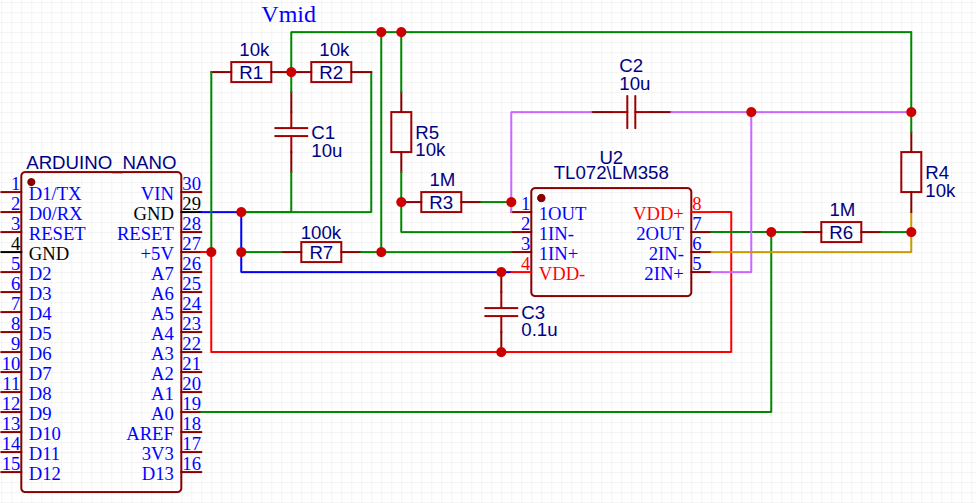
\includegraphics[width=0.93\linewidth,keepaspectratio]{pandoc_media/media/thermal_three_exp/schematic_dual_stage.png}
  \caption{Структура стенда усиления шума резистора и подключение к Arduino Nano (виртуальная середина $V_\mathrm{mid}$, два неинвертирующих каскада, выход на A0)}
  \label{fig:thermal_schematic}
\end{figure}

\textbf{3.3.2. Совокупный шум на входе и на выходе: откуда вклад}

Реальный сигнал перед АЦП --- не «чистый» шум одного резистора $100$~кОм. К
входу-повторителю добавляются статистически независимые (в идеале) вклады:
\textbf{(а)} напряжение теплового шума $R_\mathrm{noise}$ и тепловой шум сопоставимых
сопротивлений в цепочке к $V_\mathrm{mid}$; \textbf{(б)} входной \textit{напряжённый}
и \textit{токовый} шум операционника (во многих датчиках bipolar-input он заметнее,
чем для низкошумного JFET-усилителя); \textbf{(в)} вклад больших резисторов $R_{f1}$
и $R_{f2}$, чья собственная тепловая напряжённость пересчитывается к входу обратной
связи и при высоких $R_{f1}$, $R_{f2}$ становится конкурентной теплу $100$~кОм;
\textbf{(г)} наводки и микрофонность монтажа при ослабленной развязке; \textbf{(д)}
несовершенство развязки питания (частично компенсируют $10$ и $0{,}1$~мкФ); \textbf{(е)}
неточность полосы усиления: спектр на выходе окрашен, поэтому нельзя просто умножить
$40$~нВ$/\sqrt{\mathrm{Гц}}$ на корень из номинальной частоты Найквиста без учёта
изометрии АЦП, фильтрации конденсаторами и полюсов ОУ/макета. Поэтому \textbf{оценить
действующее напряжение шума на выходе}, сверив только с теорией для одного резистора,
некорректно: нужно хотя бы сопоставить \textit{порядки}: при $R=100$~кОм плотность
$\sim 40$~нВ$/\sqrt{\mathrm{Гц}}$ на входе усиления; при узкой полосе $\Delta f$ чисто
резисторный вклад на выходе имел бы порядок $G_1 G_2\,e_{\mathrm{n},R}\sqrt{\Delta f}$,
однако реальная СПМ на АЦП обычно выше за счёт перечисленных источников и неравномерной
полосы --- что и видно по различию трёх экспериментов.

\textbf{3.3.3. Номиналы трёх постановок и расчёт усиления}

Во всех трёх опытах сохранялись: $R_\mathrm{noise}=100$~кОм; $R_{g1}=R_{g2}=10$~кОм;
$R_{f2}=1$~МОм; конденсаторы $10$~мкФ, $10$~мкФ, $0{,}1$~мкФ по назначению, описанному
выше. Различия --- в таблице~\ref{tab:thermal_setups}.

\begin{table}[htbp]
  \centering
  \footnotesize
  \caption{Варианты теплового эксперимента и расчётные коэффициенты усиления}
  \label{tab:thermal_setups}
  \begin{tabular}{|p{0.14\linewidth}|p{0.16\linewidth}|c|c|c|c|}
    \hline
    Опыт & ОУ & $R_{f1}$ & $G_1$ & $G_2$ & $G_1 G_2$ \\
    \hline
    1 & LM358 & $1$~МОм & $101$ & $101$ & $\approx 1{,}02\cdot 10^4$ \\
    \hline
    2 & TL072 & $1$~МОм & $101$ & $101$ & $\approx 1{,}02\cdot 10^4$ \\
    \hline
    3 & LM358 & $10$~МОм & $1001$ & $101$ & $\approx 1{,}01\cdot 10^5$ \\
    \hline
  \end{tabular}
\end{table}

Третий опыт носит \textbf{сравнительный} характер: при $R_{f1}=10$~МОм линейная модель
на всей полосе перестаёт быть надёжной --- растут риск насыщения, влияние токов смещения,
самовозбуждения и широкополосных артефактов; форма спектра и гистограмма отражают уже
\textbf{совокупность} шумов и нелинейностей на большом усилении, а не «эталонный»
резисторный Johnson в изолированном виде.

\textbf{3.3.4. Результаты измерений и интерпретация}

Регистрация велась на прошивке канала теплового шума с частотой дискретизации АЦП
порядка $76{,}9$~кГц; для каждого варианта накоплены выборки по $N=85\cdot 10^6$
отсчётов, построены гистограмма, спектр и автокорреляции, выполнены извлечение МЗР,
постобработка по схеме фон Неймана и прогон NIST STS версии $2{,}1{,}2$.
Формат сводных таблиц совпадает с описанием колонок для акустического канала
(таблицы~\ref{tab:nist_lsb},~\ref{tab:nist_vn}); для теплового канала полные сводки по
всем трём постановкам приведены ниже.

\begin{table}[htbp]
  \centering
  \footnotesize
  \caption{Сводная статистика сырого АЦП и медиана СПМ (частота пика в спектральной оценке Уэлча)}
  \label{tab:thermal_results}
  \begin{tabular}{|c|p{0.12\linewidth}|c|c|c|c|}
    \hline
    Опыт & Выборочное среднее & $\sigma_{\mathrm{adc}}$ & $\chi^2$ (равн. корз.) & медиана СПМ & пик, Гц \\
    \hline
    1 (LM358) & $537{,}9$ & $15{,}7$ & $1{,}57\cdot 10^9$ & $8{,}1\cdot 10^{-5}$ & $\approx 225$ \\
    \hline
    2 (TL072) & $429{,}4$ & $3{,}81$ & $6{,}91\cdot 10^9$ & $4{,}1\cdot 10^{-6}$ & $\approx 75$ \\
    \hline
    3 (LM358 $10$~МОм) & $536{,}2$ & $55{,}6$ & $5{,}0\cdot 10^8$ & $2{,}0\cdot 10^{-4}$ & $\approx 28$ \\
    \hline
  \end{tabular}
\end{table}

На рисунках~\ref{fig:thermal_hist_three} и~\ref{fig:thermal_autocorr_three} показаны
гистограммы отсчётов АЦП и нормированная автокорреляционная функция для всех трёх
вариантов аппаратной конфигурации.

\begin{figure}[htbp]
  \centering
  \footnotesize
  \begin{minipage}[t]{0.31\linewidth}
    \centering
    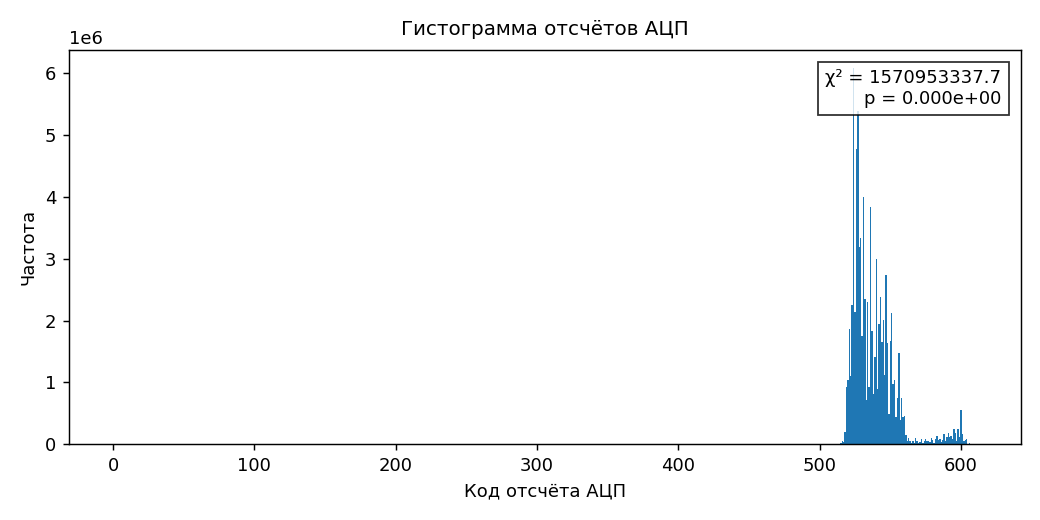
\includegraphics[width=\linewidth,keepaspectratio]{pandoc_media/media/thermal_three_exp/plots/exp1_histogram_raw.png}\\[0.4ex]
    а)~LM358, $R_{f1}=1$~МОм
  \end{minipage}\hfill
  \begin{minipage}[t]{0.31\linewidth}
    \centering
    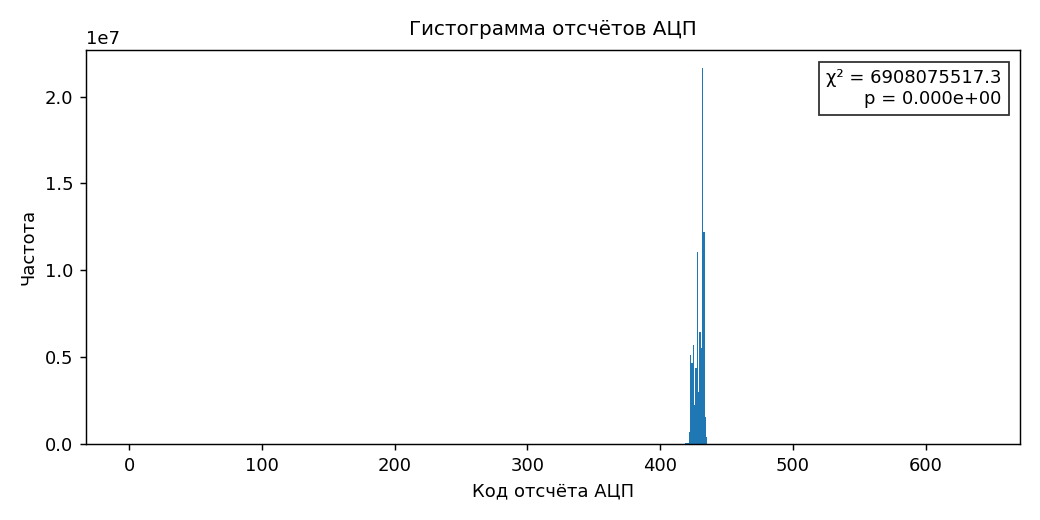
\includegraphics[width=\linewidth,keepaspectratio]{pandoc_media/media/thermal_three_exp/plots/exp2_histogram_raw.png}\\[0.4ex]
    б)~TL072, $R_{f1}=1$~МОм
  \end{minipage}\hfill
  \begin{minipage}[t]{0.31\linewidth}
    \centering
    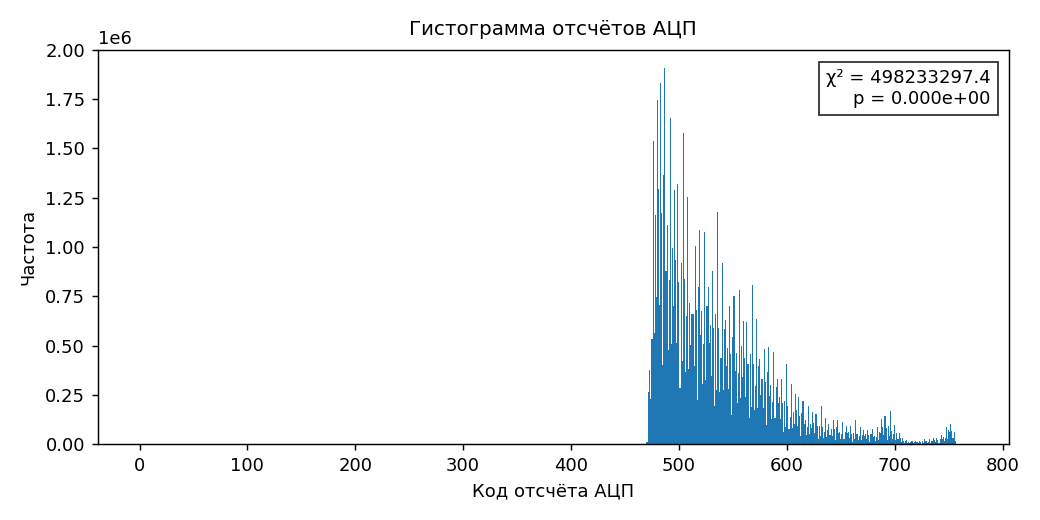
\includegraphics[width=\linewidth,keepaspectratio]{pandoc_media/media/thermal_three_exp/plots/exp3_histogram_raw.png}\\[0.4ex]
    в)~LM358, $R_{f1}=10$~МОм
  \end{minipage}
  \caption{Гистограммы отсчётов АЦП ($N=85\cdot10^6$) для трёх постановок теплового канала}
  \label{fig:thermal_hist_three}
\end{figure}

\begin{figure}[htbp]
  \centering
  \footnotesize
  \begin{minipage}[t]{0.31\linewidth}
    \centering
    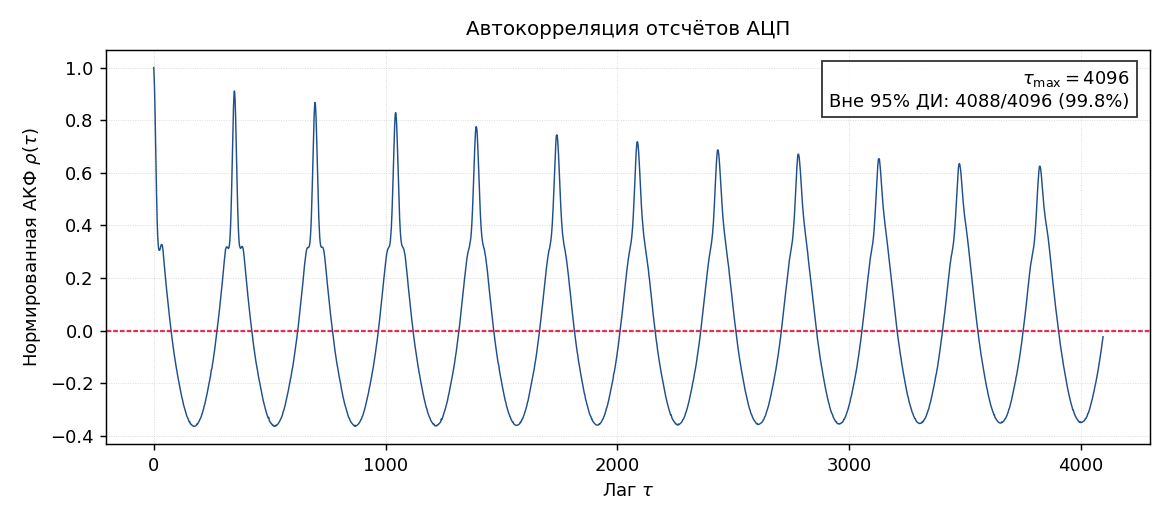
\includegraphics[width=\linewidth,keepaspectratio]{pandoc_media/media/thermal_three_exp/plots/exp1_autocorr_raw.png}\\[0.4ex]
    а)~LM358, $R_{f1}=1$~МОм
  \end{minipage}\hfill
  \begin{minipage}[t]{0.31\linewidth}
    \centering
    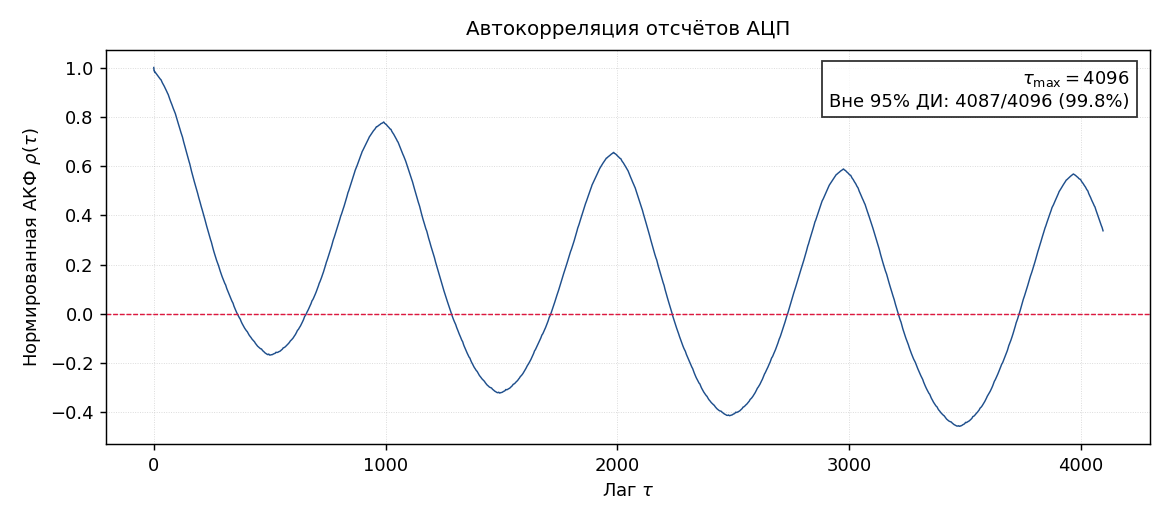
\includegraphics[width=\linewidth,keepaspectratio]{pandoc_media/media/thermal_three_exp/plots/exp2_autocorr_raw.png}\\[0.4ex]
    б)~TL072, $R_{f1}=1$~МОм
  \end{minipage}\hfill
  \begin{minipage}[t]{0.31\linewidth}
    \centering
    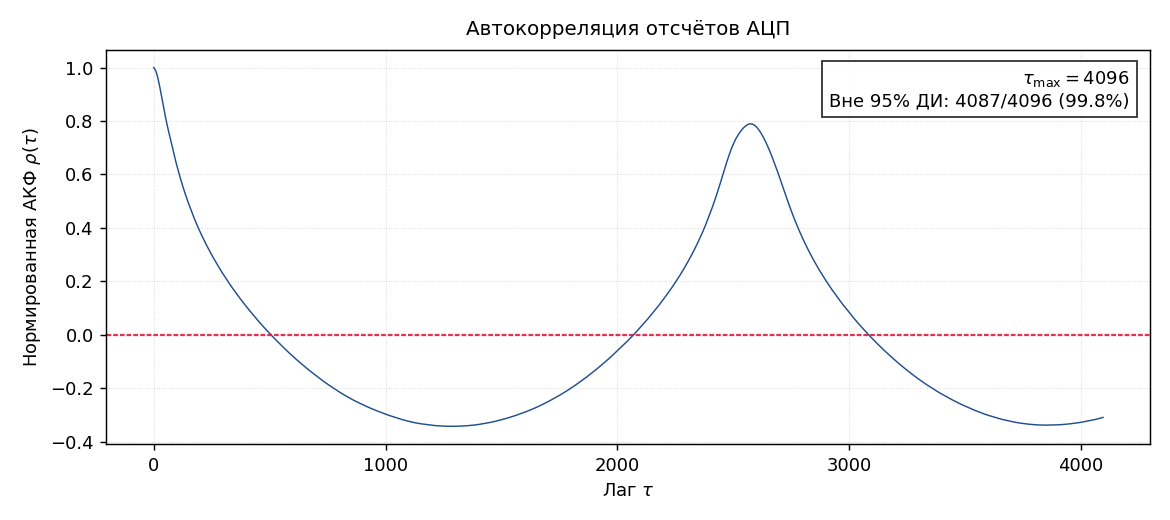
\includegraphics[width=\linewidth,keepaspectratio]{pandoc_media/media/thermal_three_exp/plots/exp3_autocorr_raw.png}\\[0.4ex]
    в)~LM358, $R_{f1}=10$~МОм
  \end{minipage}
  \caption{Автокорреляция отсчётов АЦП для трёх постановок теплового канала}
  \label{fig:thermal_autocorr_three}
\end{figure}

\textbf{Разброс средних и дисперсий.} Среднее по шкале отсчётов задаёт общий уровень
смещения относительно $V_\mathrm{mid}$ после каскадов и калибровки АЦП; при опытах с
разными ОУ оно изменяется (например, опыт 2 против 1 --- разные входные токи смещения и
режим второго усилителя). Дисперсия $\sigma_{\mathrm{adc}}$ характеризует ширину
работающего шумового «облака» на входе преобразователя: после замены LM358 на TL072 при
\textbf{тех же номиналах} она упала более чем в четыре раза, что согласуется с более
низкой типовой напряжённостью входного шума и более широкой полосой у «тихих» входов по
JFET против «бюджетного» bipolar-усиления LM358 при одинаковом расчётном $G_1 G_2$.

В третьем случае дисперсия резко \textbf{возрастает}: экстремальное усиление
усиливает не только вклад резистора, но и любые синфазные и дифференциальные помехи;
пик спектра смещается к ещё более низкой частоте, спектральная медиана растёт --- это
\textbf{совместимо} с включением бóльших низкочастотных и широкополосных компонент
(композиций нескольких источников), а не с одним узкополосным белым процессом.

\textbf{NIST STS.} Для оценённых битовых потоков полный профиль тестов остаётся
преимущественно с отрицательным вердиктом во всех трёх постановках: это ожидаемо для
простых выходов аппаратуры без специализированного криптографического усиления. При этом
\textbf{конфигурируются по-разному} относительные успехи: для опытов после фон Неймана
число групп с PASS равнялось соответственно четырём и четырем для опытов 1 и 2, но
\textbf{лишь двум} для опыта с $10$~МОм (при числе FAIL, равном $13$ против $11$ для
первых двух) --- избыточное усиление ухудшило наблюдаемую случайность с точки зрения
набора STS. Одновременно нельзя приравнивать «больше
напряжения шума» к «выше качество энтропии»: третья постановка наглядно показывает
компромисс между видимым размахом сигнала и сохранением структуры, допустимой для
стандартных тестов случайности. Детализация по группам тестов для каждого опыта приведена
в таблицах~\ref{tab:thermal_exp1_nist_lsb}--\ref{tab:thermal_exp3_nist_vn}.

\begin{table}[htbp]
  \centering
  \footnotesize
  \caption{NIST STS (МЗР без фон Неймана). Опыт 1: LM358, $R_{f1}=1$~МОм.
    Сводка: PASS${}=2$, FAIL${}=11$, N/A${}=2$.}
  \label{tab:thermal_exp1_nist_lsb}
  \begin{tabular}{|p{0.34\linewidth}|r|r|r|c|}
    \hline
    Группа тестов & Под\-тестов & min / max $p$ & Пройдено / всего & Вердикт \\
    \hline
    Frequency & 1 & $0{,}0000$ & $0/10$ & FAIL \\
    \hline
    BlockFrequency & 1 & $0{,}0000$ & $0/10$ & FAIL \\
    \hline
    CumulativeSums & 2 & $0{,}0000$ -- $0{,}0000$ & $0/20$ & FAIL \\
    \hline
    Runs & 1 & $0{,}0000$ & $0/10$ & FAIL \\
    \hline
    LongestRun & 1 & $0{,}0000$ & $4/10$ & FAIL \\
    \hline
    Rank & 1 & $0{,}7399$ & $10/10$ & PASS \\
    \hline
    FFT & 1 & $0{,}0000$ & $0/10$ & FAIL \\
    \hline
    NonOverlappingTemplate & 148 & $0{,}0000$ -- $0{,}9114$ & $508/1480$ & FAIL \\
    \hline
    OverlappingTemplate & 1 & $0{,}0000$ & $0/10$ & FAIL \\
    \hline
    Universal & 1 & $0{,}0000$ & $0/10$ & FAIL \\
    \hline
    ApproximateEntropy & 1 & $0{,}0000$ & $0/10$ & FAIL \\
    \hline
    RandomExcursions & 8 & --- & --- & N/A \\
    \hline
    RandomExcursionsVariant & 18 & --- & --- & N/A \\
    \hline
    Serial & 2 & $0{,}0000$ -- $0{,}0043$ & $10/20$ & FAIL \\
    \hline
    LinearComplexity & 1 & $0{,}7399$ & $10/10$ & PASS \\
    \hline
  \end{tabular}
\end{table}

\begin{table}[htbp]
  \centering
  \footnotesize
  \caption{NIST STS (после фон Неймана). Опыт 1: LM358, $R_{f1}=1$~МОм.
    Сводка: PASS${}=4$, FAIL${}=11$, N/A${}=0$.}
  \label{tab:thermal_exp1_nist_vn}
  \begin{tabular}{|p{0.34\linewidth}|r|r|r|c|}
    \hline
    Группа тестов & Под\-тестов & min / max $p$ & Пройдено / всего & Вердикт \\
    \hline
    Frequency & 1 & $0{,}5341$ & $9/10$ & PASS \\
    \hline
    BlockFrequency & 1 & $0{,}0000$ & $0/10$ & FAIL \\
    \hline
    CumulativeSums & 2 & $0{,}2133$ -- $0{,}7399$ & $18/20$ & PASS \\
    \hline
    Runs & 1 & $0{,}0000$ & $0/10$ & FAIL \\
    \hline
    LongestRun & 1 & $0{,}0000$ & $0/10$ & FAIL \\
    \hline
    Rank & 1 & $0{,}5341$ & $10/10$ & PASS \\
    \hline
    FFT & 1 & $0{,}0000$ & $5/10$ & FAIL \\
    \hline
    NonOverlappingTemplate & 148 & $0{,}0000$ -- $0{,}9114$ & $404/1480$ & FAIL \\
    \hline
    OverlappingTemplate & 1 & $0{,}0000$ & $0/10$ & FAIL \\
    \hline
    Universal & 1 & $0{,}0000$ & $0/10$ & FAIL \\
    \hline
    ApproximateEntropy & 1 & $0{,}0000$ & $0/10$ & FAIL \\
    \hline
    RandomExcursions & 8 & --- & $33/40$ & FAIL \\
    \hline
    RandomExcursionsVariant & 18 & --- & $90/90$ & FAIL \\
    \hline
    Serial & 2 & $0{,}0000$ -- $0{,}7399$ & $10/20$ & FAIL \\
    \hline
    LinearComplexity & 1 & $0{,}3505$ & $10/10$ & PASS \\
    \hline
  \end{tabular}
\end{table}

\begin{table}[htbp]
  \centering
  \footnotesize
  \caption{NIST STS (МЗР без фон Неймана). Опыт 2: TL072, $R_{f1}=1$~МОм.
    Сводка: PASS${}=1$, FAIL${}=12$, N/A${}=2$.}
  \label{tab:thermal_exp2_nist_lsb}
  \begin{tabular}{|p{0.34\linewidth}|r|r|r|c|}
    \hline
    Группа тестов & Под\-тестов & min / max $p$ & Пройдено / всего & Вердикт \\
    \hline
    Frequency & 1 & $0{,}0000$ & $0/10$ & FAIL \\
    \hline
    BlockFrequency & 1 & $0{,}0000$ & $0/10$ & FAIL \\
    \hline
    CumulativeSums & 2 & $0{,}0000$ -- $0{,}0000$ & $0/20$ & FAIL \\
    \hline
    Runs & 1 & $0{,}0000$ & $0/10$ & FAIL \\
    \hline
    LongestRun & 1 & $0{,}0000$ & $0/10$ & FAIL \\
    \hline
    Rank & 1 & $0{,}0000$ & $0/10$ & FAIL \\
    \hline
    FFT & 1 & $0{,}0000$ & $0/10$ & FAIL \\
    \hline
    NonOverlappingTemplate & 148 & $0{,}0000$ -- $0{,}9114$ & $80/1480$ & FAIL \\
    \hline
    OverlappingTemplate & 1 & $0{,}0000$ & $0/10$ & FAIL \\
    \hline
    Universal & 1 & $0{,}0000$ & $0/10$ & FAIL \\
    \hline
    ApproximateEntropy & 1 & $0{,}0000$ & $0/10$ & FAIL \\
    \hline
    RandomExcursions & 8 & --- & --- & N/A \\
    \hline
    RandomExcursionsVariant & 18 & --- & --- & N/A \\
    \hline
    Serial & 2 & $0{,}0000$ -- $0{,}0000$ & $0/20$ & FAIL \\
    \hline
    LinearComplexity & 1 & $0{,}3505$ & $10/10$ & PASS \\
    \hline
  \end{tabular}
\end{table}

\begin{table}[htbp]
  \centering
  \footnotesize
  \caption{NIST STS (после фон Неймана). Опыт 2: TL072, $R_{f1}=1$~МОм.
    Сводка: PASS${}=4$, FAIL${}=11$, N/A${}=0$.}
  \label{tab:thermal_exp2_nist_vn}
  \begin{tabular}{|p{0.34\linewidth}|r|r|r|c|}
    \hline
    Группа тестов & Под\-тестов & min / max $p$ & Пройдено / всего & Вердикт \\
    \hline
    Frequency & 1 & $0{,}7399$ & $10/10$ & PASS \\
    \hline
    BlockFrequency & 1 & $0{,}0000$ & $0/10$ & FAIL \\
    \hline
    CumulativeSums & 2 & $0{,}7399$ -- $0{,}9114$ & $20/20$ & PASS \\
    \hline
    Runs & 1 & $0{,}0000$ & $0/10$ & FAIL \\
    \hline
    LongestRun & 1 & $0{,}0000$ & $0/10$ & FAIL \\
    \hline
    Rank & 1 & $0{,}7399$ & $10/10$ & PASS \\
    \hline
    FFT & 1 & $0{,}0000$ & $0/10$ & FAIL \\
    \hline
    NonOverlappingTemplate & 148 & $0{,}0000$ -- $0{,}7399$ & $84/1480$ & FAIL \\
    \hline
    OverlappingTemplate & 1 & $0{,}0000$ & $0/10$ & FAIL \\
    \hline
    Universal & 1 & $0{,}0000$ & $0/10$ & FAIL \\
    \hline
    ApproximateEntropy & 1 & $0{,}0000$ & $0/10$ & FAIL \\
    \hline
    RandomExcursions & 8 & --- & $8/27$ & FAIL \\
    \hline
    RandomExcursionsVariant & 18 & --- & $90/90$ & FAIL \\
    \hline
    Serial & 2 & $0{,}0000$ -- $0{,}0000$ & $0/20$ & FAIL \\
    \hline
    LinearComplexity & 1 & $0{,}7399$ & $10/10$ & PASS \\
    \hline
  \end{tabular}
\end{table}

\begin{table}[htbp]
  \centering
  \footnotesize
  \caption{NIST STS (МЗР без фон Неймана). Опыт 3: LM358, $R_{f1}=10$~МОм.
    Сводка: PASS${}=2$, FAIL${}=11$, N/A${}=2$.}
  \label{tab:thermal_exp3_nist_lsb}
  \begin{tabular}{|p{0.34\linewidth}|r|r|r|c|}
    \hline
    Группа тестов & Под\-тестов & min / max $p$ & Пройдено / всего & Вердикт \\
    \hline
    Frequency & 1 & $0{,}0000$ & $0/10$ & FAIL \\
    \hline
    BlockFrequency & 1 & $0{,}0000$ & $0/10$ & FAIL \\
    \hline
    CumulativeSums & 2 & $0{,}0000$ -- $0{,}0000$ & $0/20$ & FAIL \\
    \hline
    Runs & 1 & $0{,}0000$ & $0/10$ & FAIL \\
    \hline
    LongestRun & 1 & $0{,}0000$ & $0/10$ & FAIL \\
    \hline
    Rank & 1 & $0{,}0352$ & $10/10$ & PASS \\
    \hline
    FFT & 1 & $0{,}0000$ & $1/10$ & FAIL \\
    \hline
    NonOverlappingTemplate & 148 & $0{,}0000$ -- $0{,}9114$ & $346/1480$ & FAIL \\
    \hline
    OverlappingTemplate & 1 & $0{,}0000$ & $0/10$ & FAIL \\
    \hline
    Universal & 1 & $0{,}0000$ & $0/10$ & FAIL \\
    \hline
    ApproximateEntropy & 1 & $0{,}0000$ & $0/10$ & FAIL \\
    \hline
    RandomExcursions & 8 & --- & --- & N/A \\
    \hline
    RandomExcursionsVariant & 18 & --- & --- & N/A \\
    \hline
    Serial & 2 & $0{,}0000$ -- $0{,}0000$ & $0/20$ & FAIL \\
    \hline
    LinearComplexity & 1 & $0{,}5341$ & $10/10$ & PASS \\
    \hline
  \end{tabular}
\end{table}

\begin{table}[htbp]
  \centering
  \footnotesize
  \caption{NIST STS (после фон Неймана). Опыт 3: LM358, $R_{f1}=10$~МОм.
    Сводка: PASS${}=2$, FAIL${}=13$, N/A${}=0$.}
  \label{tab:thermal_exp3_nist_vn}
  \begin{tabular}{|p{0.34\linewidth}|r|r|r|c|}
    \hline
    Группа тестов & Под\-тестов & min / max $p$ & Пройдено / всего & Вердикт \\
    \hline
    Frequency & 1 & $0{,}3505$ & $8/10$ & FAIL \\
    \hline
    BlockFrequency & 1 & $0{,}0000$ & $0/10$ & FAIL \\
    \hline
    CumulativeSums & 2 & $0{,}2133$ -- $0{,}3505$ & $16/20$ & FAIL \\
    \hline
    Runs & 1 & $0{,}0000$ & $0/10$ & FAIL \\
    \hline
    LongestRun & 1 & $0{,}0000$ & $0/10$ & FAIL \\
    \hline
    Rank & 1 & $0{,}9114$ & $10/10$ & PASS \\
    \hline
    FFT & 1 & $0{,}0000$ & $0/10$ & FAIL \\
    \hline
    NonOverlappingTemplate & 148 & $0{,}0000$ -- $0{,}9114$ & $247/1480$ & FAIL \\
    \hline
    OverlappingTemplate & 1 & $0{,}0000$ & $0/10$ & FAIL \\
    \hline
    Universal & 1 & $0{,}0000$ & $0/10$ & FAIL \\
    \hline
    ApproximateEntropy & 1 & $0{,}0000$ & $0/10$ & FAIL \\
    \hline
    RandomExcursions & 8 & --- & $27/40$ & FAIL \\
    \hline
    RandomExcursionsVariant & 18 & --- & $90/90$ & FAIL \\
    \hline
    Serial & 2 & $0{,}0000$ -- $0{,}3505$ & $10/20$ & FAIL \\
    \hline
    LinearComplexity & 1 & $0{,}3505$ & $10/10$ & PASS \\
    \hline
  \end{tabular}
\end{table}

\textbf{Вывод раздела.} Расчётные коэффициенты усиления $G_1$, $G_2$ совпадают с
назначением резисторов в неинвертирующих каскадах и объясняют возрастающую амплитуду во
\textbf{второй} номинальной точке только по линейной части. Наблюдаемые действующие значения и
формы распределений \textbf{не сводятся} к простой подстановке $e_{\mathrm{n},100\mathrm{k}\Omega}$
на произведение $G_1 G_2$: решающее значение имеют тип ОУ ($1/f$, ток шума, полоса
усиления), тепловой шум мегомных резисторов обратной связи при пересчёте к входу,
наводки и выбранный режим эксперимента третий как искусственно «нагружающий» канал без
ретуши нелинейностей --- что полезно для критической интерпретации применения
дешёвого аналога в роли генератора случайности.

\textbf{3.4. Экспериментальная оценка акустического источника энтропии на
базе электретного микрофона}

Идея использовать акустический канал в качестве физического входа генератора
истинно случайных последовательностей не нова: на её основе описывают как
учебные прототипы, так и специализированные постановки, где цифровой звуковой
вход служит источником хаотически смешанных колебаний среды и собственных
шумов аппаратуры. При этом сам по себе факт наличия «шума» у микрофона не
делает выходную двоичную последовательность пригодной для криптографии:
необходимо учитывать полосу и форму спектра, устойчивую временную
корреляцию отсчётов аналого-цифрового преобразователя (АЦП), неравномерность
распределения амплитуд после квантования, а также возможные узкополосные
составляющие сетевых наводок и механических резонансов. Перечисленные эффекты
особенно заметны в компактной конструкции на базе микроконтроллера, где вход
АЦП соединён с модулем микрофона коротким жгутом без экранирования и без
развязки по постоянному току промышленного уровня.

Натурная часть работы выполнялась в бытовых условиях: регистрация велась в
обычной комнате многоквартирного кирпичного дома при естественном акустическом
фоне без специально организованного шумового воздействия и без акустической
камеры. Уровень окружающего звука оценивается как умеренный (тишина,
редкие бытовые шумы соседних помещений), что приближает эксперимент к типичному
сценарию использования низкобюджетного модуля «на столе», но одновременно
означает доминирование структурированных и слабо контролируемых составляющих
над «идеальным» белым шумом.

В качестве первичного преобразователя использован модуль KY-037 с электретным
капсюлем и операционным усилителем с регулируемой чувствительностью; выход
аналогового сигнала подключался непосредственно ко входу АЦП микроконтроллера
семейства Arduino. Рабочая точка усилителя выставлялась в середине диапазона
напряжения питания, чтобы модуляция от акустических событий происходила в
линейной области без клиппирования. Дискретизация выполнялась на частоте
около $38461$~Гц при разрешении $10$ бит (полный диапазон АЦП); выбор такой
скорости определяется конфигурацией предделителя тактов АЦП и обеспечивает
компромисс между охватом аудиополосы и объёмом записываемых данных.

\begin{figure}[htbp]
  \centering
  \noindent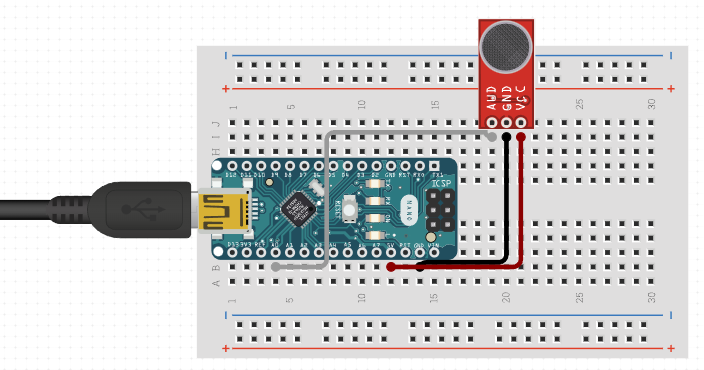
\includegraphics[width=0.92\linewidth,keepaspectratio]{pandoc_media/media/trng_microphone/microphone_wiring.png}
  \caption{Подключение модуля KY-037 к плате Arduino: выход \textit{AO} модуля соединён с аналоговым входом АЦП, питание --- от шины платы}
  \label{fig:mic_wiring}
\end{figure}

Сеанс накопления данных выполнялся по последовательному интерфейсу UART при
скорости линии $10^6$~бод; метаданные записи фиксируют переданный объём сырых
данных в формате «младший байт первым» (\textit{uint16 little-endian}), без
пропусков и без аварийного прерывания. Из объёма и длительности сеанса следуют
средние скорости поступления информации на стороне приёника и эффективная частота
отсчётов с учётом реального времени передачи (она несколько ниже номинальной
частоты дискретизации АЦП из-за протокольных служебных символов и программных
задержек приёмника). Для того же интервала времени вычислены средние скорости
битового потока после извлечения МЗР и после постобработки по схеме фон Неймана
(таблица~\ref{tab:mic_capture}).

\begin{table}[htbp]
  \centering
  \footnotesize
  \caption{Параметры сеанса записи акустического канала и производные скорости}
  \label{tab:mic_capture}
  \begin{tabular}{|p{0.52\linewidth}|p{0.38\linewidth}|}
    \hline
    Объём сырых данных (последовательность 16-битных отсчётов) & $170\cdot10^6$ байт \\
    \hline
    Число отсчётов АЦП & $85\cdot10^6$ \\
    \hline
    Длительность захвата (по временным меткам приёмника) & $2225{,}46$~с (${\approx}37{,}09$~мин) \\
    \hline
    Средняя скорость приёма по UART & ${\approx}7{,}64\cdot10^4$ байт/с (${\approx}74{,}6$ КиБ/с) \\
    \hline
    Эффективная частота отсчётов по длительности сеанса & ${\approx}3{,}82\cdot10^4$~Гц \\
    \hline
    Номинальная частота дискретизации в прошивке & $38461$~Гц \\
    \hline
    Объём упакованных бит после извлечения МЗР & ${\approx}1{,}06\cdot10^7$ байт (${\approx}85\cdot10^6$ бит) \\
    \hline
    Средняя скорость потока МЗР & ${\approx}3{,}82\cdot10^4$ бит/с \\
    \hline
    Объём после схемы фон Неймана & ${\approx}2{,}10\cdot10^6$ байт (${\approx}1{,}68\cdot10^7$ бит) \\
    \hline
    Средняя скорость после фон Неймана & ${\approx}7{,}55\cdot10^3$ бит/с \\
    \hline
    Доля выходных бит фон Неймана от числа бит МЗР за сеанс & ${\approx}19{,}8\,\%$ \\
    \hline
  \end{tabular}
\end{table}

Теоретический потолок полезной передачи при $10^6$~бод и типичном кадрировании
UART заметно выше достигнутой средней скорости по таблице~\ref{tab:mic_capture};
фактический результат ограничивается форматом кадра протокола обмена с платой,
накладными расходами на синхронизацию и производительностью цепочки «АЦП ---
передача --- запись на хост», что видно по разнице между номинальной частотой
АЦП и эффективной частотой отсчётов, усреднённой по длительности всего сеанса.

Для получения двоичной последовательности из потока отсчётов применялось
извлечение младшего значащего разряда (МЗР, LSB) каждого отсчёта. Такой приём
часто используют как простейший способ концентрироваться на локальной
случайности младших бит при условии, что источник не насыщен и не имеет
выраженной периодичности на уровне младших разрядов. Дополнительно изучался
вариант постобработки по схеме фон Неймана для ослабления статистического
смещения (несимметрии вероятностей нуля и единицы): из пар последовательных
бит сохраняются только несовпадающие пары \((01)\rightarrow 0\),
\((10)\rightarrow 1\), совпадающие отбрасываются. Отметим, что схема фон Неймана
устраняет смещение при допущении независимости пар бит и не является
«универсальной» процедурой криптографического усиления: она не устраняет
последовательную зависимость и не заменяет экстракторы, опирающиеся на
хэширование или решёточные методы.

Оценка качества потока проводилась в двух дополняющих друг друга направлениях.
Во-первых, анализировались статистические свойства самих отсчётов АЦП и
полученных из них битовых последовательностей (гистограмма, автокорреляция,
спектральная плотность мощности, оценки энтропии на символ по методике,
согласованной с подходами NIST SP~800-90B к минимальной энтропии на один
выходной символ). Во-вторых, выполнялась верификация пакетом NIST Statistical
Test Suite (STS) версии 2.1.2 для двух файлов: последовательность МЗР без
постобработки фон Неймана и последовательность после постобработки. Использовался
типовой режим группового вердикта по подтестам (несколько независимых двоичных
потоков фиксированной длины); интерпретация результатов опирается на долю
потоков, прошедших тест при заданном пороге значимости для \textit{p-value}.

На рисунках \ref{fig:mic_hist}, \ref{fig:mic_acf_raw} и~\ref{fig:mic_psd} приведены гистограмма
отсчётов, нормированная автокорреляционная функция и оценка спектральной плотности
мощности сигнала на входе АЦП. На рисунке~\ref{fig:mic_bits_map} приведена карта
первых $40000$ бит потока после схемы фон Неймана ($200\times200$ пикселей,
каждый пиксель соответствует одному биту); на рисунке~\ref{fig:mic_acf_bits} ---
автокорреляция всего доступного битового массива после постобработки.

\begin{figure}[htbp]
  \centering
  \noindent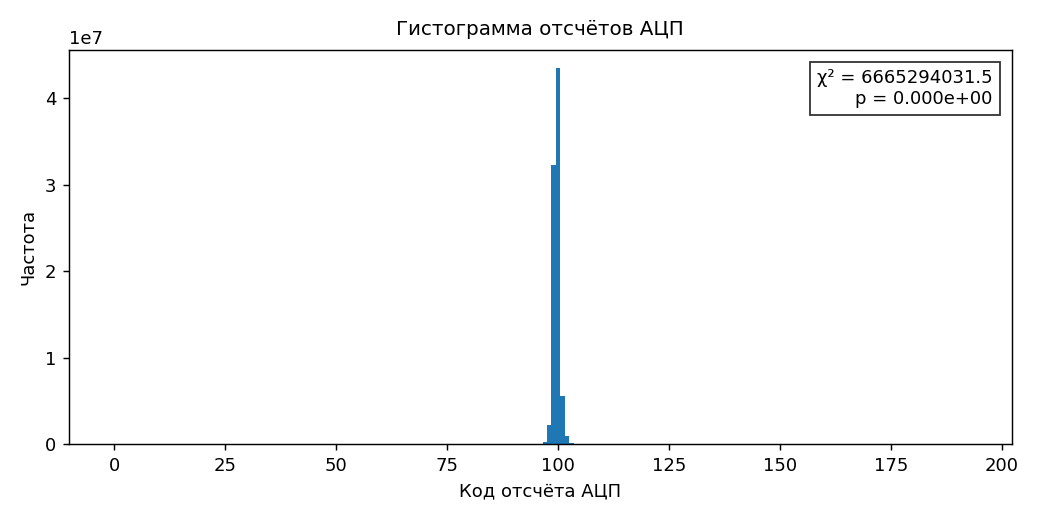
\includegraphics[width=\linewidth,keepaspectratio]{pandoc_media/media/trng_microphone/histogram_raw.png}
  \caption{Гистограмма распределения отсчётов АЦП для акустического канала}
  \label{fig:mic_hist}
\end{figure}

\begin{figure}[htbp]
  \centering
  \noindent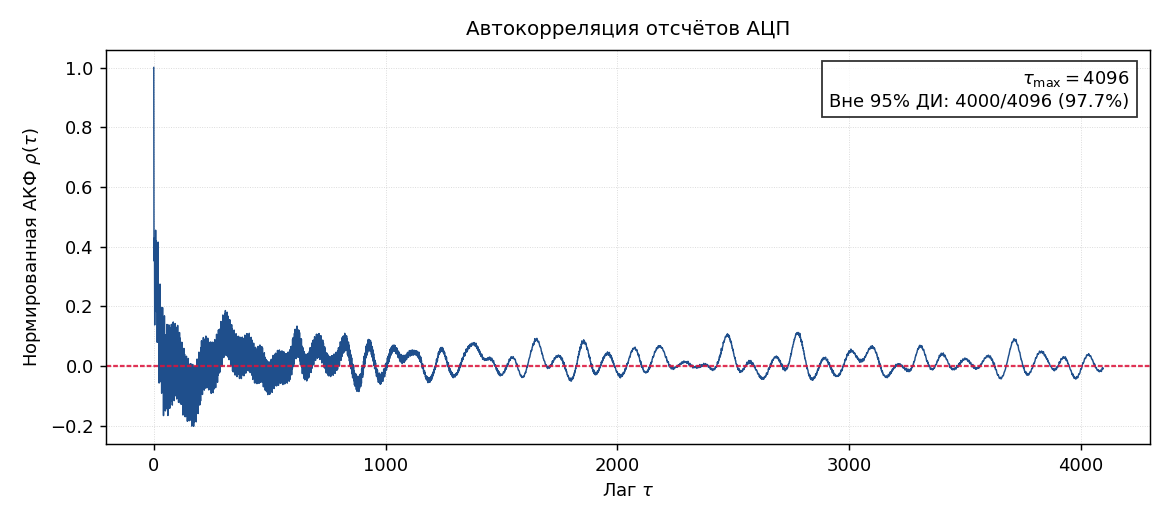
\includegraphics[width=\linewidth,keepaspectratio]{pandoc_media/media/trng_microphone/autocorr_raw.png}
  \caption{Автокорреляция отсчётов АЦП (временная зависимость)}
  \label{fig:mic_acf_raw}
\end{figure}

\begin{figure}[htbp]
  \centering
  \noindent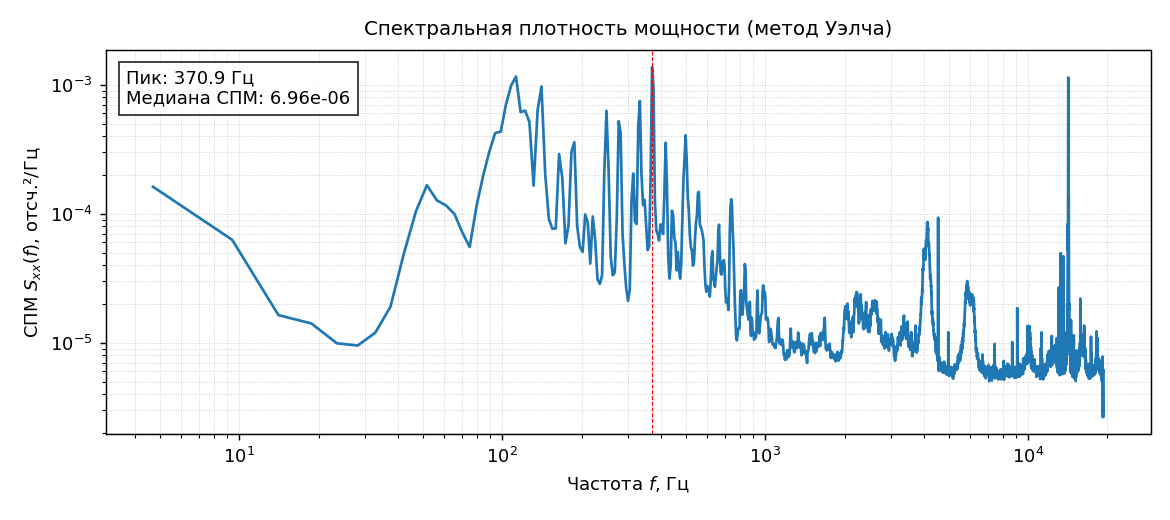
\includegraphics[width=\linewidth,keepaspectratio]{pandoc_media/media/trng_microphone/psd_raw.png}
  \caption{Оценка спектральной плотности мощности входного сигнала}
  \label{fig:mic_psd}
\end{figure}

\begin{figure}[htbp]
  \centering
  \noindent
\includegraphics[width=0.52\linewidth,keepaspectratio]{pandoc_media/media/trng_microphone/bits_map_200x200.png}
  \caption{Визуализация первых $40000$ бит после извлечения МЗР и постобработки по схеме фон Неймана (матрица $200\times200$ пикселей; белый --- единица, чёрный --- ноль)}
  \label{fig:mic_bits_map}
\end{figure}

\begin{figure}[htbp]
  \centering
  \noindent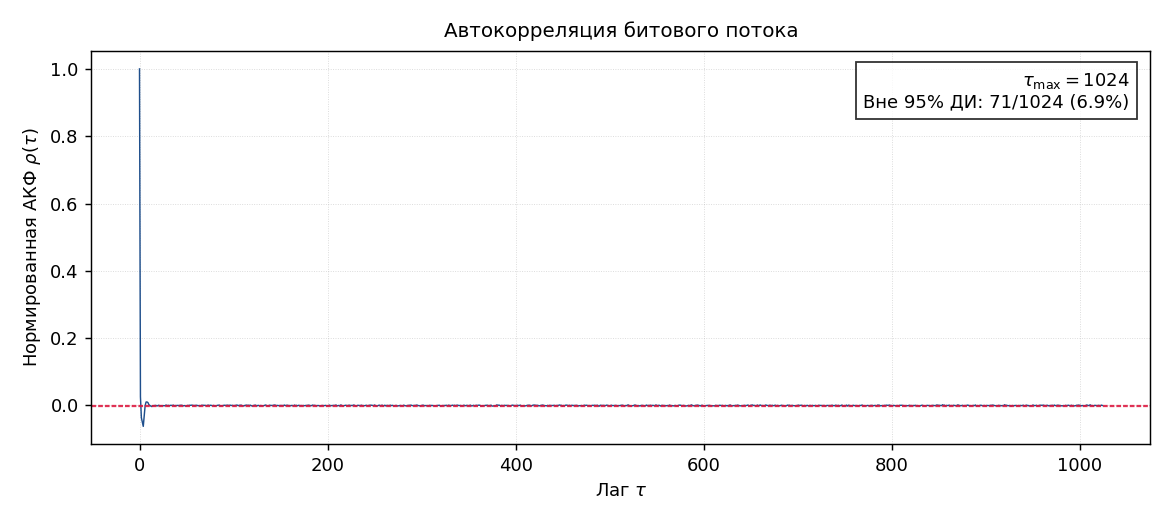
\includegraphics[width=\linewidth,keepaspectratio]{pandoc_media/media/trng_microphone/autocorr_bits.png}
  \caption{Автокорреляция битового потока после постобработки по схеме фон Неймана}
  \label{fig:mic_acf_bits}
\end{figure}

\begin{table}[htbp]
  \centering
  \footnotesize
  \caption{Сводные показатели сырого АЦП-сигнала (конечная выборка эксперимента)}
  \label{tab:mic_raw_stats}
  \begin{tabular}{|p{0.52\linewidth}|p{0.38\linewidth}|}
    \hline
    Число отсчётов $N$ & $85\cdot10^6$ \\
    \hline
    Выборочное среднее & $99{,}65$ \\
    \hline
    Стандартное отклонение & $0{,}90$ \\
    \hline
    Минимум / максимум по выборке & $80$ / $192$ \\
    \hline
    Критерий согласия Пирсона $\chi^2$ (равномерность по корзинам) & $\approx 6{,}67\cdot10^9$ \\
    \hline
    Достигаемый уровень значимости & $\approx 0$ \\
    \hline
  \end{tabular}
\end{table}

\begin{table}[htbp]
  \centering
  \footnotesize
  \caption{Спектральные характеристики по оценке Уэлча}
  \label{tab:mic_psd_stats}
  \begin{tabular}{|p{0.52\linewidth}|p{0.38\linewidth}|}
    \hline
    Эффективная частота дискретизации $f_s$ & $38461$~Гц \\
    \hline
    Частота пика спектральной плотности & $\approx 370{,}9$~Гц \\
    \hline
    Медиана спектральной плотности мощности & $\approx 6{,}96\cdot10^{-6}$ \\
    \hline
  \end{tabular}
\end{table}

\begin{table}[htbp]
  \centering
  \footnotesize
  \caption{Оценки энтропии на символ для постобработанной последовательности (фон Нейман)}
  \label{tab:mic_entropy}
  \begin{tabular}{|p{0.34\linewidth}|c|c|}
    \hline
    Показатель & На бит & На байт ($8$ бит) \\
    \hline
    Пер-битовая энтропия Шеннона & $1{,}0000$ & $7{,}9687$ \\
    \hline
    Минимальная энтропия (min-entropy) & $0{,}9994$ & $7{,}0447$ \\
    \hline
    min-entropy по частоте наиболее вероятного символа (MCV, SP~800-90B §6.3.1) & $0{,}9985$ & $7{,}0157$ \\
    \hline
  \end{tabular}
\end{table}

Гистограмма отсчётов и результат теста на равномерность показывают, что даже при
«тишине» в бытовой комнате распределение уровней на входе АЦП концентрируется в
узком диапазоне около установленной средней точки усилителя (таблица
\ref{tab:mic_raw_stats}). На практике это означает, что канал работает как
узкополосный процесс с большим постоянным уровнем и небольшой амплитудой флуктуаций,
а не как источник, равномерно занимающий доступную шкалу квантования. Такое поведение
ожидаемо для недорогого аналогового тракта без автоматической регулировки усиления:
энергия акустического фона оказывается мала по сравнению с доступным динамическим
диапазоном, а доминирующая доля изменений связана с дробовым шумом электроники,
наводками и неидеальностью развязки по постоянному току.

Автокорреляционная функция отсчётов (рисунок \ref{fig:mic_acf_raw}) выявляет
выраженную память процесса: значимые значения коэффициентов сохраняются на больших
лагах относительно типичной для белого шума «δ-подобной» формы. Это согласуется с
наличием узкой полосы и фильтрующих свойств входного тракта АЦП и буфера выборки,
а также с тем, что спектр содержит выраженную гармоническую составляющую (таблица
\ref{tab:mic_psd_stats}, рисунок \ref{fig:mic_psd}). Частота пика порядка сотен
герц при типичном фоне без организованного акустического возмущения может отражать
совокупность электромагнитных и механических источников (в том числе наводки на
компоненты модуля и проводники), при этом её точное атрибутирование выходит за рамки
наблюдательной постановки; для задачи генерации случайности критичен сам факт
наличия устойчивой узкополосной компоненты, делает ли её более предсказуемым спектр
битового потока и проваливает спектральный тест случайности.

Извлечение МЗР на фоне узкой гистограммы и заметной автокорреляции приводит к
последовательности бит с выраженными статистическими дефектами: классические тесты
на долю единиц и нулей, блоковые частотные тесты, серийные характеристики и другие
проверки чувствительны как к несимметрии, так и к скрытой периодичности и локальной
повторяемости паттернов. Это качественно подтверждается результатами NIST STS для
файла МЗР без схемы фон Неймана (таблица \ref{tab:nist_lsb}): вердикты большинства
групп тестов отрицательные; исключение составляют тест ранга двоичной матрицы и тест
линейной сложности, которые менее чувствительны к тем типам отклонений, которые
доминируют в данном канале. Для части профилей Random Excursions программа вернула
статус недоступности результата (N/A), что согласуется с ограничениями постановки:
при крайнем отклонении распределений относительных долей единиц и нулей от идеальных
предпосылок отдельные статистики могут быть численно неустойчивы или не формализуются
стандартным шаблоном расчёта.

После применения схемы фон Неймана распределение по крайнему символу становится
ближе к симметричному на уровне одиночных битов, что проявляется, например, в
«ровной» карте битового потока (рисунок \ref{fig:mic_bits_map}) и значительном
ослаблении первых коэффициентов автокорреляции бит (рисунок \ref{fig:mic_acf_bits}).
Табличные оценки энтропии на символ (таблица \ref{tab:mic_entropy}) близки к
номинальным значениям для непрерывной шкалы при условии интерпретации как верхней
границы по наблюдаемым частотам; однако высокая минимальная энтропия на байте по
сравнению с границей Шеннона отражает наличие повторяющихся байтовых шаблонов,
неизбежных при сохранении временной структуры исходного процесса даже после
устранения простейшего смещения.

Результаты NIST STS после фон Неймана (таблица \ref{tab:nist_vn}) показывают частичное
улучшение: проходят глобальный частотный тест и тест на кумулятивные суммы отклонений,
устойчиво проходит тест ранга матрицы; тест линейной сложности получает групповой
вердикт PASS при том, что один из десяти двоичных потоков не удовлетворяет критерию по
\textit{p-value}. Вместе с тем сохраняются провалы в
блоковом частотном тесте (единичный поток из десяти не удовлетворяет критерию),
что типично при наличии локальной регулярности долей единиц и нулей внутри длинных
блоков. Провалы тестов серий, наибольших серий единиц, спектрального (FFT), шаблонных,
универсального Мауриса, приблизительной энтропии и серийных тестов указывают на
сохраняющуюся зависимость между битами и наличие повторяемых паттернов длиной,
сравнимой с параметрами тестов. Тесты случайных экскурсий и их вариант после
постобработки получили численные результаты по всем подпотокам, однако суммарный групповой вердикт
для обеих групп остаётся отрицательным: даже при формально полном покрытии подпотоков отдельные статистики выходят за
допустимые границы распределений при множественном тестировании. Таким образом, хотя постобработка по
фон Нейману исправляет наиболее грубое проявление несимметрии и улучшает отдельные
глобальные метрики, она не переводит канал в класс последовательностей, проходящих
полный профиль STS без дополнительных мер.

Практический вывод для инженерной постановки состоит в следующем. Акустический вход на
базе недорогого модуля микрофона в условиях обычной комнаты при простейшем извлечении
МЗР не может рассматриваться как самостоятельный криптографический источник без
узкой специализации тракта (развязка, фильтрация, управление коэффициентом усиления,
возможно, смешение нескольких независимых физических каналов) и без последующего
криптографического постпроцессора с доказуемыми свойствами экстракции. При этом канал
оставляется показательным учебным объектом: он наглядно демонстрирует разницу между
«наличием шума на осциллографе» и выполнением формализованных статистических требований,
а также иллюстрирует ограничения локальных методов устранения смещения в условиях
сильной временной корреляции и узкополосных составляющих.

Уточним структуру сводных таблиц~\ref{tab:nist_lsb} и~\ref{tab:nist_vn}. По каждой
\textit{группе} теста (одна строка) перечисляется число \textit{подтестов} --- отдельных
настроек внутри процедуры assess (разные шаблоны для NonOverlappingTemplate, два
направления для Cumulative Sums и Serial и т.\,д.). Колонка \textit{min / max}
$p$ задаёт минимальный и максимальный среди подтестов этой группы \textit{сводный}
\textit{p-value}, который STS выносит во вторую фазу оценки (проверка согласованности с
равномерностью распределений по корзинам); при единственном подтесте указывается одно
значение, при полном отсутствии числовых $p$-value ставится прочерк. Колонка
\textit{пройдено / всего} суммирует \textit{первый уровень} проверки: сколько двоичных
потоков из серии экспериментальных последовательностей удовлетворили индивидуальному
критерию успешности по каждому подтесту, суммированному по строке группы.

\begin{table}[htbp]
  \centering
  \footnotesize
  \caption{Сводка NIST STS для последовательности МЗР без схемы фон Неймана}
  \label{tab:nist_lsb}
  \begin{tabular}{|p{0.36\linewidth}|r|r|r|c|}
    \hline
    Группа тестов & Под\-тестов & min / max $p$ & Пройдено / всего & Вердикт \\
    \hline
    Frequency & 1 & $0{,}0000$ & $0/10$ & FAIL \\
    \hline
    BlockFrequency & 1 & $0{,}0000$ & $0/10$ & FAIL \\
    \hline
    CumulativeSums & 2 & $0{,}0000$ -- $0{,}0000$ & $0/20$ & FAIL \\
    \hline
    Runs & 1 & $0{,}0000$ & $0/10$ & FAIL \\
    \hline
    LongestRun & 1 & $0{,}0000$ & $0/10$ & FAIL \\
    \hline
    Rank & 1 & $0{,}5341$ & $10/10$ & PASS \\
    \hline
    FFT & 1 & $0{,}0000$ & $0/10$ & FAIL \\
    \hline
    NonOverlappingTemplate & 148 & $0{,}0000$ -- $0{,}0000$ & $9/1480$ & FAIL \\
    \hline
    OverlappingTemplate & 1 & $0{,}0000$ & $0/10$ & FAIL \\
    \hline
    Universal & 1 & $0{,}0000$ & $0/10$ & FAIL \\
    \hline
    ApproximateEntropy & 1 & $0{,}0000$ & $0/10$ & FAIL \\
    \hline
    RandomExcursions & 8 & --- & --- & N/A \\
    \hline
    RandomExcursionsVariant & 18 & --- & --- & N/A \\
    \hline
    Serial & 2 & $0{,}0000$ -- $0{,}0000$ & $0/20$ & FAIL \\
    \hline
    LinearComplexity & 1 & $0{,}3505$ & $10/10$ & PASS \\
    \hline
  \end{tabular}
\end{table}

\begin{table}[htbp]
  \centering
  \footnotesize
  \caption{Сводка NIST STS для последовательности после схемы фон Неймана}
  \label{tab:nist_vn}
  \begin{tabular}{|p{0.36\linewidth}|r|r|r|c|}
    \hline
    Группа тестов & Под\-тестов & min / max $p$ & Пройдено / всего & Вердикт \\
    \hline
    Frequency & 1 & $0{,}3505$ & $10/10$ & PASS \\
    \hline
    BlockFrequency & 1 & $0{,}0000$ & $9/10$ & FAIL \\
    \hline
    CumulativeSums & 2 & $0{,}7399$ -- $0{,}9114$ & $20/20$ & PASS \\
    \hline
    Runs & 1 & $0{,}0000$ & $0/10$ & FAIL \\
    \hline
    LongestRun & 1 & $0{,}0000$ & $2/10$ & FAIL \\
    \hline
    Rank & 1 & $0{,}5341$ & $10/10$ & PASS \\
    \hline
    FFT & 1 & $0{,}0000$ & $0/10$ & FAIL \\
    \hline
    NonOverlappingTemplate & 148 & $0{,}0000$ -- $0{,}0089$ & $264/1480$ & FAIL \\
    \hline
    OverlappingTemplate & 1 & $0{,}0000$ & $0/10$ & FAIL \\
    \hline
    Universal & 1 & $0{,}0000$ & $0/10$ & FAIL \\
    \hline
    ApproximateEntropy & 1 & $0{,}0000$ & $0/10$ & FAIL \\
    \hline
    RandomExcursions & 8 & --- & $40/48$ & FAIL \\
    \hline
    RandomExcursionsVariant & 18 & --- & $108/108$ & FAIL \\
    \hline
    Serial & 2 & $0{,}0000$ -- $0{,}0000$ & $5/20$ & FAIL \\
    \hline
    LinearComplexity & 1 & $0{,}5341$ & $9/10$ & PASS \\
    \hline
  \end{tabular}
\end{table}

\textbf{3.5. Перспективные направления развития физических генераторов
случайных последовательностей (ФГСП)}

Современные требования к безопасности информационных систем, а также
рост применения криптографических и статистических методов в различных
областях обуславливают необходимость дальнейшего совершенствования
физических генераторов случайных последовательностей (ФГСП). Развитие
данных систем направлено на повышение их надёжности, устойчивости к
внешним воздействиям, скорости генерации и интеграции в современные
аппаратные платформы. Ниже рассмотрены ключевые направления развития.

Миниатюризация и интеграция в чипы. Современные технологии производства
микросхем позволяют встраивать элементы ФГСП непосредственно в
процессоры, контроллеры и криптографические сопроцессоры. Это
обеспечивает минимальные задержки при получении случайных битов и
упрощает защиту от атак на уровне интерфейсов. Развитие технологии CMOS,
FinFET и перспективных материалов способствует созданию компактных,
энергоэффективных и массовых решений.

Перспективным направлением является использование квантовых источников
энтропии -- в частности, спонтанного распада фотонов, квантовых
флуктуаций вакуума и эффекта туннелирования. Такие источники обладают
высокой степенью истинной случайности, подтверждаемой теорией квантовой
неопределённости, и демонстрируют устойчивость к предсказуемости со
стороны атакующего. Разработка доступных и стабильно работающих
квантовых ФГСП, увеличение скорости их генерации остаются важной
задачей.

Оптические и фотонные источники также могут быть подвержены
модернизации. Оптические ФГСП, основанные на фотоэлектрическом шуме,
колебаниях интенсивности лазерного излучения и спонтанном рассеянии
света, демонстрируют высокую пропускную способность и низкую
коррелированность выходных битов. Развитие интегральной фотоники и
кремниевых фотонных чипов позволяет создавать компактные и
масштабируемые оптические генераторы с высокой скоростью и надёжностью.

Повышение надёжности генерации достигается за счёт объединения
нескольких физических источников энтропии в гибридной архитектуре.
Комбинация теплового, дробового, лавинного шумов, а также оптических и
квантовых источников позволяет компенсировать слабости отдельных
компонентов, а также реализовать адаптивные схемы оценки качества и
селекции наиболее надёжных источников в реальном времени. Таким образом,
перспективным направлением развития является изучение комбинаций
источников энтропии в ФГСП: многоканальные и гибридные схемы.

Совершенствование методов постобработки, внедрение постобработки на
аппаратном уровне также являются современной тенденцией развития ФГСП.
Для повышения энтропийной насыщенности и устранения смещения (bias)
усиливается внимание к аппаратной реализации алгоритмов экстракции,
таких как схема фон Неймана, хэш-функции и решёточные методы. Аппаратная
реализация постобработки позволяет достичь высокой скорости и
энергоэффективности без ущерба для статистических свойств выходных
данных.

Современные подходы к верификации и мониторингу работы ФГСП
предусматривают встраивание модулей контроля, способных выполнять
непрерывное статистическое тестирование и выявление деградации качества
энтропии. Это особенно важно в критических приложениях, где отклонения в
характеристиках могут привести к серьёзным уязвимостям. С появлением
новых способов атаки на ФГСП также появляется необходимость в
поддержании эффективного автоматического тестирования и самодиагностики.

В рамках международных инициатив (например, NIST, ISO) разрабатываются
единые подходы к оценке качества ФГСП. Это способствует унификации
требований, повышению доверия к устройствам и упрощению их внедрения в
сертифицированные системы безопасности.

В совокупности данные направления определяют вектор дальнейших
исследований и разработок в области ФГСП, ориентируясь на создание
высоконадёжных, воспроизводимых и проверяемых источников истинной
случайности для современных и перспективных информационно-технических
систем.

